\documentclass[12pt]{article} 

%?? paths
\newcommand{\CiteMathPackage}{../../math} 
\newcommand{\CiteReference}{../reference.bib}

%?? packages 
\usepackage{setspace,geometry,fancyvrb,rotating} 
\usepackage{marginnote,datetime,enumitem} 
\usepackage{titlesec,indentfirst} 
\usepackage{amsmath,amsfonts,amssymb,amsthm,mathtools} 
\usepackage{threeparttable,booktabs,adjustbox} 
\usepackage{graphicx,epstopdf,float,soul,subfig} 
\usepackage[toc,page]{appendix} 
\usdate

%?? page setup 
\geometry{scale=0.8} 
\titleformat{\paragraph}[runin]{\itshape}{}{}{}[.] 
\titlelabel{\thetitle.\;} 
\setlength{\parindent}{10pt} 
\setlength{\parskip}{10pt} 
\usepackage{Alegreya} 
\usepackage[T1]{fontenc}

%?? bibliography 
\usepackage{natbib,fancybox,url,xcolor} 
\definecolor{MyBlue}{rgb}{0,0.2,0.6} 
\definecolor{MyRed}{rgb}{0.4,0,0.1} 
\definecolor{MyGreen}{rgb}{0,0.4,0} 
\definecolor{MyPink}{HTML}{E50379} 
\definecolor{MyOrange}{HTML}{FF5733} 
\definecolor{MyPurple}{HTML}{BF40BF}
\newcommand{\highlightR}[1]{{\emph{\color{MyRed}{#1}}}} 
\newcommand{\highlightB}[1]{{\emph{\color{MyBlue}{#1}}}} 
\newcommand{\highlightP}[1]{{\emph{\color{MyPink}{#1}}}} 
\newcommand{\highlightO}[1]{{\emph{\color{MyOrange}{#1}}}}
\newcommand{\highlightPP}[1]{{\emph{\color{MyPurple}{#1}}}}
\usepackage[bookmarks=true,bookmarksnumbered=true,colorlinks=true,linkcolor=MyBlue,citecolor=MyRed,filecolor=MyBlue,urlcolor=MyGreen]{hyperref} \bibliographystyle{econ}

%?? math and theorem environment 
\theoremstyle{definition} 
\newtheorem{assumption}{Assumption} 
\newtheorem{definition}{Definition} 
\newtheorem{theorem}{Theorem} 
\newtheorem{proposition}{Proposition} 
\newtheorem{lemma}{Lemma} 
\newtheorem{example}{Example} 
\newtheorem{corollary}[theorem]{Corollary} 
\usepackage{mathtools} 
\usepackage{\CiteMathPackage}

\begin{document} 

%??%??%??%??%??%??%??%??%??%??%??%??%??%??%??%??%??%??%??%??%??%?? 
%?? title 
%??%??%??%??%??%??%??%??%??%??%??%??%??%??%??%??%??%??%??%??%??%??

\title{\bf Distribution of Ability and Earnings in a Hierarchical Job Assignment Model, Journal of Political Economy, 2004} 
\author{Wenzhi Wang \thanks{This note is written in my pre-doc period at the University of Chicago Booth School of Business.} } 
\date{\today} 
\maketitle 

\citet{costrellDistributionAbilityEarnings2004}

\section{Introduction}

\section{A Two-Job Model}

In this work we investigate the relationship between the distribution of workers' ability and the resulting distribution of wages that obtains in competitive equilibrium. A worker's contribution to total firm output depends on his own ability and also on the job he occupies. We begin by finding the equilibrium distribution of wages in a simple two-job model. 

The key feature of the model is that jobs must be filled in fixed proportions to one another, $\t$ and $1-\t$. Consider a world, for example, of production and supervisory jobs, with a fixed span of control. Alternatively, suppose that production takes place in terms of fixed composition, for example, two-person teams of an electrician and an electrician's helper. One may think of software teams with coders and debuggers in proportions that are hard to vary, or research teams with lead researchers and research assistants, where, again, the quantity of workers cannot be substituted for quality in one or the other type of job.

In the simplest case, output depends only on the ability of those in production jobs; support jobs generate no output, but must be filled to keep the operation going. More generally, suppose that one job is more ability-sensitive than the other, such that output per unit of ability on the two jobs is $\b_1 > \b_0 \geq 0$. Thus, $\t, \b_0, \b_1$ completely characterize the technology. 

Let $\mu \in \bs{0,1}$ denote a worker's ability (or expected ability, given available information). The distribution of ability is exogenous and is characterized by the CDF $F\of{\mu}$, so $p = F\of{\mu}$ denotes the ability quantile of a worker with ability $\mu$. Equivalently, let $\mu\of{p} \equiv F^{-1}\of{p}$ denote the ability at rank $p$. Workers will be assigned to job 1 or 0 as $\mu \gtrless \wh{\mu} \equiv \mu\of{\t}$. Output is 
\begin{equation}
    \notag 
    Q = \b_0 \int_{0}^{\t} \mu\of{p} dp + \b_1 \int_{\t}^{1} \mu\of{p} dp. 
\end{equation}

It is important to be clear on how the complementarities under consideration in this model pertain to the \highlightP{number} of workers across jobs versus their \highlightP{abilities}. Under the strict complementarity we have posited, the effect on output of adding another worker of any given ability to a given job depends very much on the \highlightP{number} of workers in the other jobs: they must remain in strict proportion. By contrast, the effect on output of raising the \highlightP{ability} of a worker in one job is assumed independent of the \highlightP{abilities} of workers in the other jobs. 

The wage schedule is derived from two conditions. The no-arbitrage condition on job assignment gives the slope of the wage function: 
$$
W\of{\mu} - W\of{\mu^{\prime}} = \b_i \bp{\mu - \mu^{\prime}},
$$
for any $\mu, \mu^{\prime}$ on job $i$. Otherwise profits could be raised by substituting one type of worker for another. The no-profit condition, 
$$
Q = \int_{0}^{1} W\of{\mu} d F\of{\mu},
$$
sets the level of the wage function. Specifically, these conditions imply 
\begin{equation}
    \label{1}
    W\of{\mu} = \b_0 \mu + \bp{1-\t} \bp{\b_1 - \b_0} \wh{\mu},\quad \mu < \wh{\mu},
\end{equation}
and 
\begin{equation}
    \label{2}
    W\of{\mu} = \b_1 \mu - \t \bp{\b_1 - \b_0} \wh{\mu}, \quad \mu \geq \wh{\mu}.
\end{equation}

These expressions have a straightforward marginal productivity interpretation. An additional worker of ability $\mu < \wh{\mu}$ adds $\b_0 \mu$ to output directly to job 0, but also allows the promotion of $1-\t$ workers to job 1. These workers will be promoted from the margin between the jobs, so they will have ability $\bp{\b_1 - \b_0} \wh{\mu}$, so this indirect contribution to output is captured in the second term of (\ref{1}). Thus low-ability workers earn more than their direct contribution to output. Similarly, an additional worker of ability $\mu > \wh{\mu}$, placed on job 1, earns less than his or her direct contribution to output, $\b_1 \mu$. The reason is that placement in job 1 requires the demotion of $\t$ workers of ability $\wh{\mu}$ to job 0, with the attendant loss of output, as reflected in the second term of (\ref{2}).

\begin{figure}[H]
    \noindent\caption{}
    \begin{center}
        \resizebox{0.7\textwidth}{!}{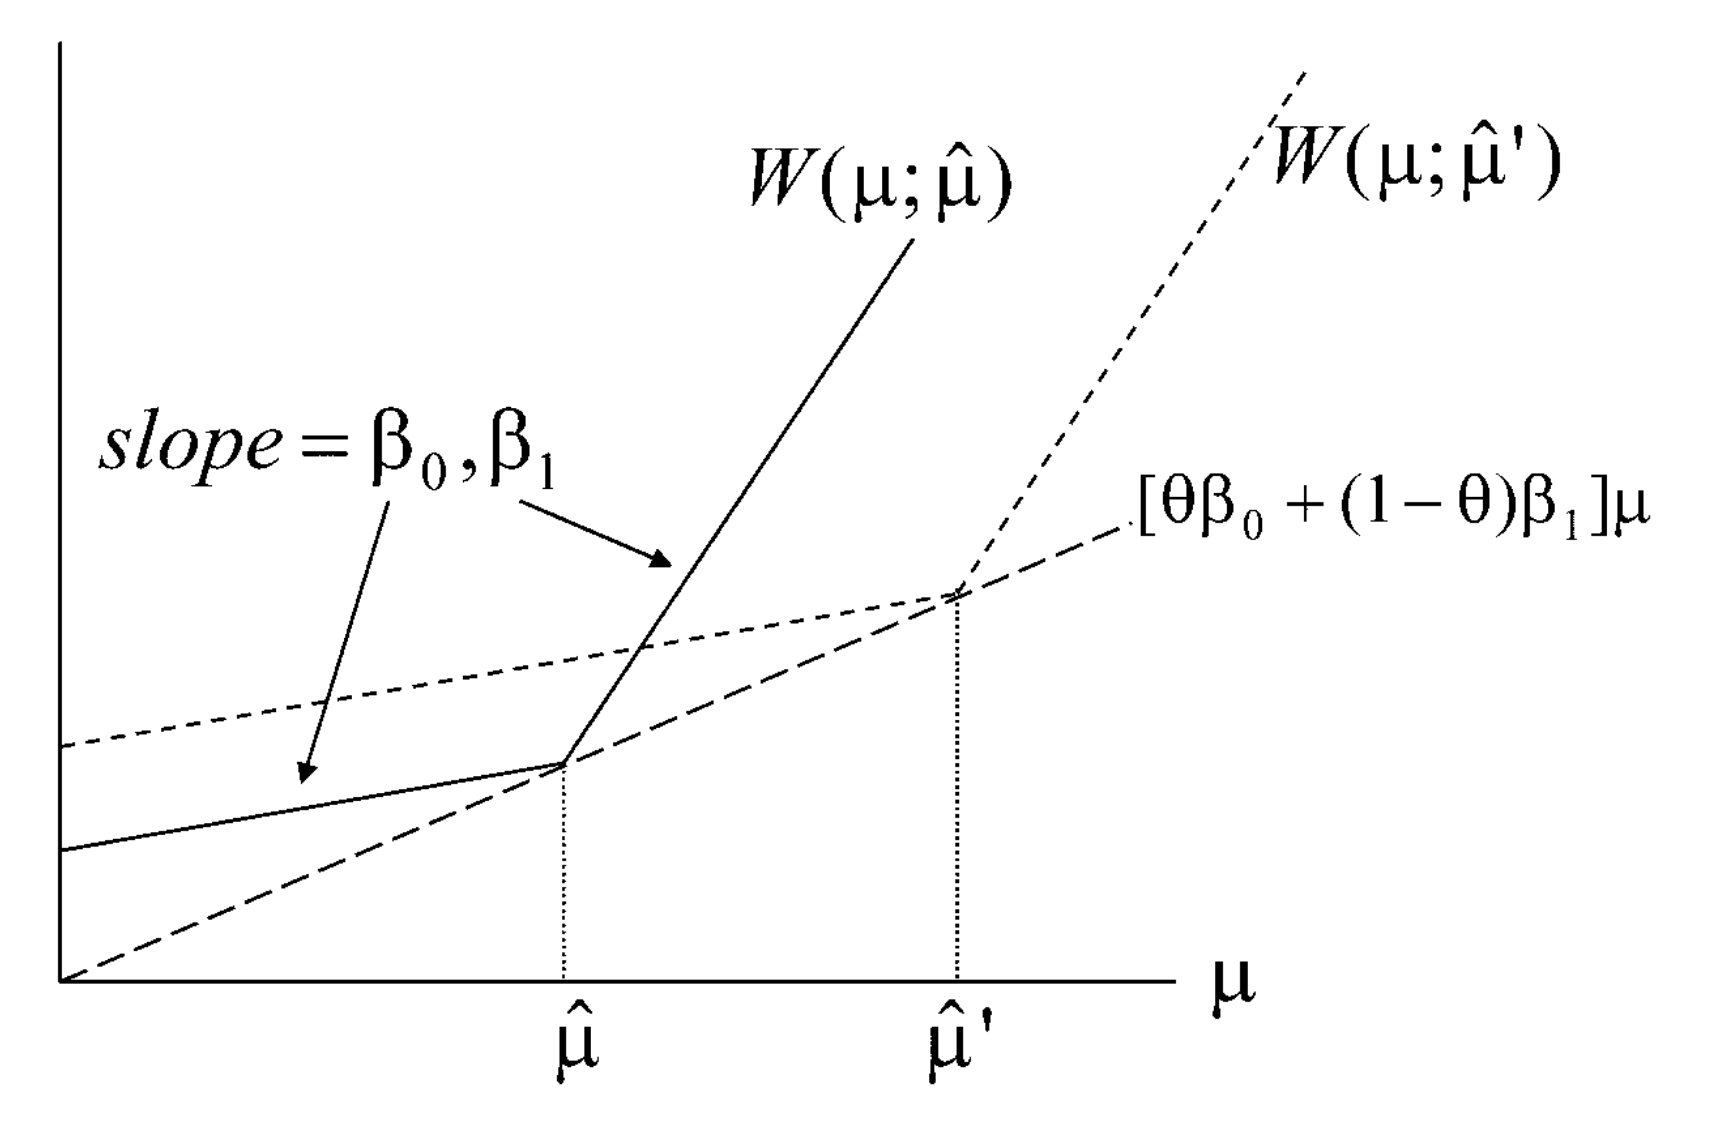
\includegraphics{costrellDistributionAbilityEarnings2004_fig1.png}}
        \label{fig1}
    \end{center}
\end{figure}



















\bibliography{\CiteReference} 

\end{document}